\documentclass[12pt,a4paper]{article}

\usepackage{polyglossia}
\setmainlanguage{french}

\usepackage{amsmath, amssymb}
\usepackage{cancel}



\usepackage{graphicx}
\usepackage{caption}

\usepackage{siunitx} % Pour les unités

\usepackage{geometry}
\geometry{top=2cm, bottom=2.5cm, left=3cm, right=3cm}
\setlength{\parindent}{0pt}

\usepackage[sfdefault]{roboto}

\usepackage{enumitem}

\usepackage{hyperref}

\usepackage{tcolorbox}
\usepackage{xcolor}

\usepackage{multicol}
\setlength{\columnseprule}{1pt}
\def\columnseprulecolor{\color{gray}}


\usepackage{import}
\usepackage{xifthen}
\usepackage{pdfpages}
\usepackage{transparent}
\usepackage{float}

\newcommand{\incfig}[1]{%
	\def\svgwidth{\columnwidth}
	\import{./figures/}{#1.pdf_tex}
}



\newcommand{\RomanNum}[1] %pour les chiffre romain
{\MakeUppercase{\romannumeral #1}}



\title{B\^{a}timent}
\author{}
\date{\today}

\begin{document}
	
	\maketitle
	\tableofcontents
	
	\newpage
	\counterwithin{section}{part} % pour que \section{} recommence de 1 aprés \part{}
	
	\part{Chapitre $\RomanNum{1}$}
	
	\part{Chapitre $\RomanNum{2}$ : Les fondations}
	
	
	
	
	\section{Les types de fondations}
	
	\begin{itemize}
		\item Fondations superficielles (Semelles isolée, profonde, Radier général).
		\item Fondations semi-profondes.
		\item Fondations profondes.
	\end{itemize}
	
	
	\section{Calcul du chargement appliquer au fondations}
	
	Avant le calcul des fondations on doit d'abord avoir les données géotechnique (Capacité portante, couche d'assise(profondeur idéale), ...ect)
	
	\vspace{\baselineskip}
	
	Pour calculer le chargement qui revient au fondation on commence par le haut du bâtiment (plancher terrasse) puis en descend (descente des charger).
	
	Le chargement est transmit par les poteaux vers les fondations, est les poteaux reprenne le chargement comme dans la figure :
	
	
	\begin{figure}[H]
		\centering
		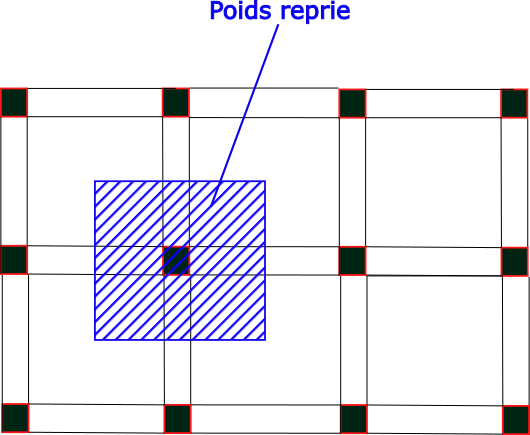
\includegraphics[width=0.5\linewidth]{figures/poids-reprie}
		\caption{Poids repris par un poteau (vue d'en haut)}
		\label{fig:poids-reprie}
	\end{figure}
	
	
	
	Pour le plancher terrasse on aura comme chargement : Le poids du corps creux, la dalle de compression, l'étanchéité, le gravier, les poutres, la charge d'exploitation si le plancher est accessible.
	
	\vspace{\baselineskip}
	
	Pour un planche courant on aura en plus le poids des revêtement, la mo\c{c}onerie et aussi le poids du poteau supérieur, charge d'exploitation, ...ect.
	l'étanchéité ne sera pas présente.
	
	
	\begin{figure}[H]
		\centering
		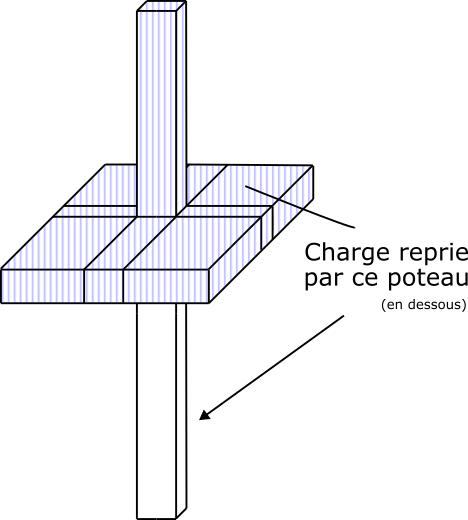
\includegraphics[width=0.5\linewidth]{figures/charge-reprie2}
		\caption{Chargement repris par le poteau dans un cas d'un plancher courant (vue de face).}
		\label{fig:charge-reprie2}
	\end{figure}
	
	
	
	\begin{tcolorbox}[colback=gray!20, colframe=black, title=Remarque]
		Dans le calcul des chargement verticale le séisme est pris en compte car ils génère les trois efforts dans le poteau(N, T, M) et aussi un effort tranchant au niveau des nœuds mais pas en mi-travée de la poutre ou bien des dalles, donc au niveau de la poutre la combinaison des charges sera sans la charge sismique(car y'aura aucun effort sismique en mi-travée de la poutre).
	\end{tcolorbox}
	
	\begin{tcolorbox}[colback=gray!20, colframe=black, title=Remarque]
		
		Les joints :
		
		\vspace{\baselineskip}
		
		On a trois type de joints : joint de dilatation thermique, sismique, rupture.
		
		Le joint de rupture est appliquer dans le cas ou on a un bâtiment construit dans deux sol différent (capacité portante différent) ou bien dans le cas ou notre bâtiment a une différence de poids par exemple du coté A on aura un R+5 et du coté B on aura R+9.
		
		Le joint de rupture permet d'éviter le tassement différentiel.
	\end{tcolorbox}
	
	
	
	
	\section{Pré-dimensionnement d'une fondation }
	
	
	\begin{figure}[H]
		
		\centering
		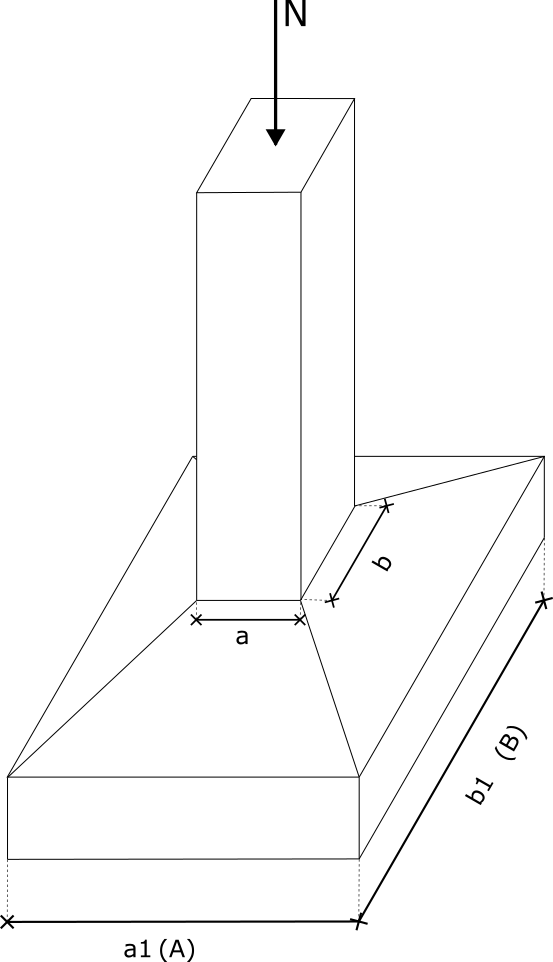
\includegraphics[width=0.4\linewidth]{figures/semelle}
		\caption{Semelle}
		\label{fig:semelle}
		
	\end{figure}
	
	
	
	\[ q \leq \sigma_{sol} \]
	
	\[ \dfrac{a}{b} = \dfrac{a_{1}}{b_{1}} \Longrightarrow a_{1} = \dfrac{a \cdot b_{1}}{b} \]
	
	\[ q = \dfrac{N}{S} = \dfrac{N}{a_{1} \cdot b_{1}} = \dfrac{N}{\dfrac{a \cdot b_{1}}{b} \cdot b_{1}} = \dfrac{N \cdot b}{a \cdot b_{1}^{2}} \]
	
	\[ q = \dfrac{N \cdot b}{a \cdot b_{1}^{2}} \Longrightarrow b_{1}^{2} = \dfrac{N \cdot b}{a \cdot q} = \dfrac{\cancel{N} \cdot b}{a \cdot \dfrac{\cancel{N}}{S}} \]
	
	\[ \text{Finalement : } \fbox{$b_{1} = \sqrt{S \cdot \dfrac{b}{a}}$} \]
	
	\[ \text{On répétant les même étapes on aura pour : } \fbox{$a_{1} = \sqrt{S \cdot \dfrac{a}{b}}$} \]
	
	\[ \fbox{$A \geq a_{1} \quad;\quad B \geq b_{1}$} \quad \text{Multiple de 5} \]
	
	\begin{tcolorbox}[colback=gray!20, colframe=black, title=Remarque]
		Pour avoir les fondations au bon emplacement avec un angle correct sur le chantier on utilise le théorème de Pythagore.
		\[ 3^{2}+4^{2} = 5^{2} \]
		
		\begin{figure}[H]
			\centering
			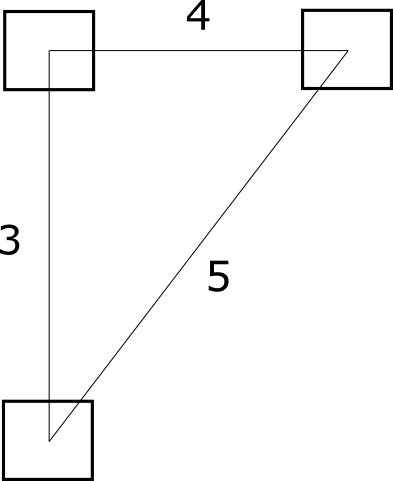
\includegraphics[width=0.3\linewidth]{figures/pythagore}
			\caption{}
			\label{fig:pythagore}
		\end{figure}
		
		
		on mesurant les distance entre axes de poteau on doit trouver les même distance ainsi on peut assurer un bon angle.
		
	\end{tcolorbox}
	
	
	
	
	
	
	
	
	\subsection{Exercice}
	
	
	
	
	Soit a vérifier une semelle \underline{\underline{\textbf{filante}}} suivante :
	
	\begin{figure}[H]
		\centering
		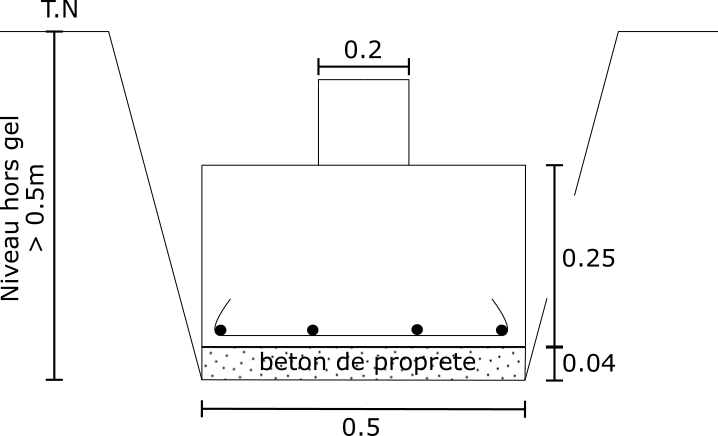
\includegraphics[width=0.7\linewidth]{figures/exercice}
		\caption{}
		\label{fig:exercice}
	\end{figure}
	
	
	\begin{itemize}
		\item Semelle filante donc 1ml de calcul.
		\item Poids volumique du béton armé : $\gamma_{ba} = 25~\unit{kN \per m^{3}}$
		\item Poids volumique du béton de propreté : $\gamma_{bp} = 22~\unit{kN \per m^{3}}$
		\item Poids volumique du sol : $\gamma_{sol} = 18~\unit{kN \per m^{3}}$
		\item Charge permanente : $G = 0,3~\unit{MN \per m}$
		\item Charge d'exploitation : $Q = 0,05~\unit{MN \per m}$
		\item Capacité portante du sol : $\sigma_{sol} = 1~\unit{MPa}$
		\item Épaisseur du béton de propreté : $e = 4~\unit{cm}$
	\end{itemize}
	
	
	\vspace{\baselineskip}
	
	On doit vérifier que : $\dfrac{N_{u}}{B \cdot 1~\unit{ml}} \leq \sigma_{sol}$
	
	\[ N_{u} = 1,35G_{tot} + 1,5Q_{tot} \]
	
	\begin{multicols}{2}
		
		\[ G_{tot} = G+G_{ba}+G_{bp}+G_{sol} \]

		Charge permanente
		
		\[ G = 0,3 \cdot 10^{3} \cdot 1 = 0,3 \cdot 10^{3}~\unit{kN} \]
		
		Poids propre du béton armé
		
		\[ G_{ba} = 25 \cdot (0,5 \cdot 0,25 \cdot 1) = 3,125~\unit{kN} \]
		
		Poids propre du béton de propreté
		
		\[ G_{bp} = 22 \cdot (0,04 \cdot 0,5 \cdot 1) = 0,44~\unit{kN} \]
		
		\columnbreak
		
		Poids propre du sol
		
		\begin{figure}[H]
			\centering
			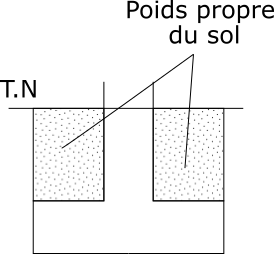
\includegraphics[width=0.5\linewidth]{figures/poids-propre-du-sol}
		\end{figure}
		
		
		\[ G_{sol} = 18 \cdot \bigg( (0,5-0,25+0,04)(0,5-0,2) \cdot 1 \bigg) \]
		\[ G_{sol} = 1,134~\unit{kN} \]
		
		Charge permanente totale
		
		\[ G_{tot} = 0,3 \cdot 10^{3}+3,125+0,44+1,134 = 304,699~\unit{kN} \]
		
		Surcharge d'exploitation
		
		\[ Q_{tot} = Q \cdot 1 = 50~\unit{kN} \]
		
		
	\end{multicols}
	
	\vspace{\baselineskip}

	\[ N_{u} = 1,35 \cdot 304,699 + 1,5 \cdot 50 = 486,34~\unit{kN} \]
	
	\[ \dfrac{N_{u}}{B \cdot 1} = \dfrac{486,34}{0,5 \cdot 1} = 972,6~\unit{kN \per m^{2}} = 0,9726~\unit{MPa} < \sigma_{sol} = 1~\unit{MPa} \quad\text{ CV }\surd \]
	
	
	\vspace{2\baselineskip}
	
	
	Maintenatn supposant que $\sigma_{sol} = 0,7~\unit{MPa}$
	
	Donc la condition n'est plus vérifier et on doit redimensinner la semelle (revoir la largeur B).
	
	\vspace{\baselineskip}
	
	\begin{multicols}{2}
		
		\[ G_{ba} = 0,25 \cdot 25 \cdot B = 6,25 \cdot B \]
		
		\[ G_{bp} = 0,04 \cdot 22 \cdot B = 0,88 \cdot B \]
		
		\columnbreak
		
		\begin{align*}
			G_{sol} &= 18 \cdot \bigg( (b-0,2) \cdot (0,5-0,29) \bigg) \\
			&= 18 \cdot (0,21 \cdot B - 0,042) \\
			&= 3,78 \cdot B -0,757
		\end{align*}
		
	\end{multicols}
	
	
	
	\[ G_{tot} = 0,3 \cdot 10^{3} + 6,25B+0,88B+3,78B-0,757 = 10,91B + 299,243 \]
	
	\[ N_{u} = 1,35G_{tot}+1,5Q_{tot} = \fbox{$14,72 \cdot B + 479$} \]
	
	\begin{align*}
		\dfrac{N_{u}}{B \cdot 1~\unit{ml}} &\leq \sigma_{sol} \\\\
		\dfrac{14,72 \cdot B + 475}{B} &\leq 0,7 \cdot 10^{3} \\
		B &\leq \dfrac{475}{685,28} \\
		B &\leq 0,692
	\end{align*}
	
	
	Finalement on choisie $B = 0,7~\unit{m}$ et on aura $q = 693,29~\unit{kN \per m^{2}} \leq \sigma_{sol}= 700~\unit{kN \per m^{2}}$ CV $\surd$
	
	
	\vspace{3\baselineskip}
	
	
	\subsection{Devoir maison}
	
	
	\begin{figure}[H]
		\centering
		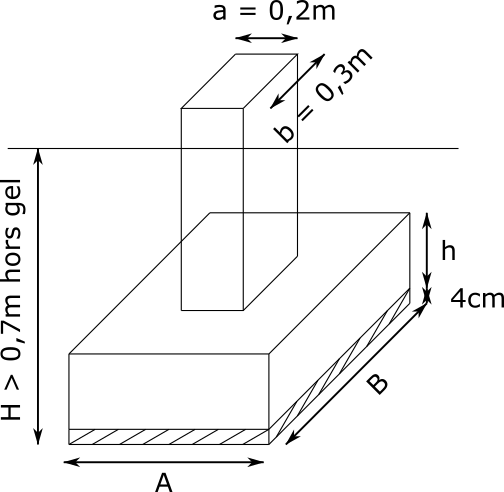
\includegraphics[width=0.5\linewidth]{figures/devoir-maison}
		\caption{}
		\label{fig:devoir-maison}
	\end{figure}
	
	
	
	\begin{itemize}
		\item $\gamma_{ba} = 25~\unit{kN \per m^{3}}$
		\item $\gamma_{bp} = 22~\unit{kN \per m^{3}}$
		\item $\gamma_{sol} = 18~\unit{kN \per m^{3}}$
		\item $G = 0,167~\unit{MN}$
		\item $Q = 0,383~\unit{MN}$
		\item $\sigma_{sol} = 0,9~\unit{MPa}$
		\item Épaisseur du BP $e = 4~\unit{cm} $
	\end{itemize}
	
	\vspace{2\baselineskip}
	
	\begin{itemize}
		\item Calculer les dimensions de la semelle isolée.
		\item Vérifier l'admissibilité de la semelle.
	\end{itemize}
	
	
	
	\vspace{\baselineskip}
	
	\subsubsection{Correction}
	
	\[ S'=0,88~\unit{m^{2}} \qquad A'= \sqrt{S' \cdot \dfrac{a}{b}} = 0,76~\unit{m} \qquad B'=\sqrt{S' \cdot \dfrac{b}{a}} = 1,15~\unit{m} \]
	
	\[ N_{u} = 1,35 \cdot G + 1,5 Q \approx 800~\unit{kN} \]
	
	
	\[ A\geq A' \qquad B\geq B' \]
	
	On choisie : $A = 0,8~\unit{m}$ et $B=1,2~\unit{m}$ $\Rightarrow S = 1,2 \cdot 0,8$
	
	\paragraph{Condition de rigidité} :
	
	\[ d_{a} \geq \dfrac{A - a}{4} = 0,15~\unit{m} \]
	
	\[ d_{b} \geq \dfrac{B - b}{4} = 0,225~\unit{m} \]
	
	
	\[ d = \max (d_{a};d_{b}) = 0,225~\unit{m} \]
	
	finalement $h = d + 0,05 = 0,225+0,05 = 0,275~\unit{m} \rightarrow 0,3~\unit{m}$
	
	
	\paragraph{Vérification de l'admissibilité de la semelle} :
	
	\[ G_{semelle+bp} = 25 \cdot (1,2 \cdot 0,8 \cdot 0,3) + 22 \cdot (1,2 \cdot 0,8 \cdot 0,04) = 8,04~\unit{kN} \]
	
	
	\[ \text{ en sachant que : } h_{sol} = 0,7-0,3-0,04 = 0,36~\unit{m} \]
	
	\[ G_{sol} = 18 \cdot \bigg( (1,2 \cdot 0,8 \cdot 0,36) - (0,2 \cdot 0,3 \cdot 0,36) \bigg) = 5,832~\unit{kN} \]
	
	\vspace{\baselineskip}
	
	\[ G_{tot} = G_{s+bp}+G_{sol} = 13,872~\unit{kN} \]
	
	\[ q_{ref} = \dfrac{N_{u}+1,35 \cdot G_{tot}}{S} = \dfrac{800 + 1,35 \cdot 13,87}{1,2 \cdot 0,8} = 852,83~\unit{kN\per m^{2}} \]
	
	
	\[ q_{ref} = 0,85~\unit{MPa} < \sigma_{sol} = 0,9~\unit{MPa} \]
	
	\[ q_{ref} = 94,44\% \cdot \sigma_{sol} \]
	
	\[ \text{Condition vérifier et semelle économique. } \surd \]
	
	
	
	
	
	
	
	
	
	
	
	
	
	
	
	
	
	
\end{document}